\documentclass{beamer}
\usepackage[ngerman]{babel}
\usepackage[ngerman]{isodate}


%\usetheme{Antibes}
\usecolortheme{default}

\title{Vuex}
\subtitle{State Management in Vue.js}
\author{Raphael Kapeller}
\date{13.05.2022}

%\usetheme{lucid}
\begin{document}
\begin{frame}
    \titlepage
\end{frame}
\begin{frame}
    \frametitle{Inhalt}
    \tableofcontents
\end{frame}

\section{Einführung}
\subsection{Was ist Vuex?}
\begin{frame}
    \frametitle{Was ist Vuex?}
    \begin{block}{Flux/State Management Pattern}
        \begin{center}
            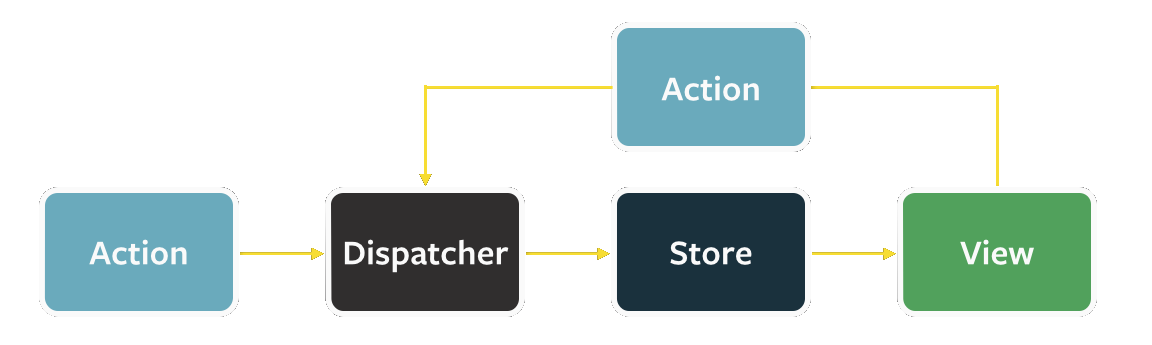
\includegraphics[scale=0.3]{flux.png}
        \end{center}
    \end{block}
    \begin{block}{für Vue.js}
        \begin{itemize}
            \item zentraler Store für alle Komponenten
            \item Regeln für Zugriffe
        \end{itemize}
    \end{block}
\end{frame}
\begin{frame}
    \frametitle{State Management Pattern}
    \begin{columns}
        \column{0.5\textwidth}
        Bestandteile
        \begin{itemize}
            \item State
            \item View
            \item Actions
        \end{itemize}
        One-Way Data Flow
        \begin{itemize}
            \item Abbildung $\rightarrow$
        \end{itemize}
        Vorteile
        \begin{itemize}
            \item Struktur
            \item Wartbarkeit
        \end{itemize}
        \column{0.5\textwidth}
        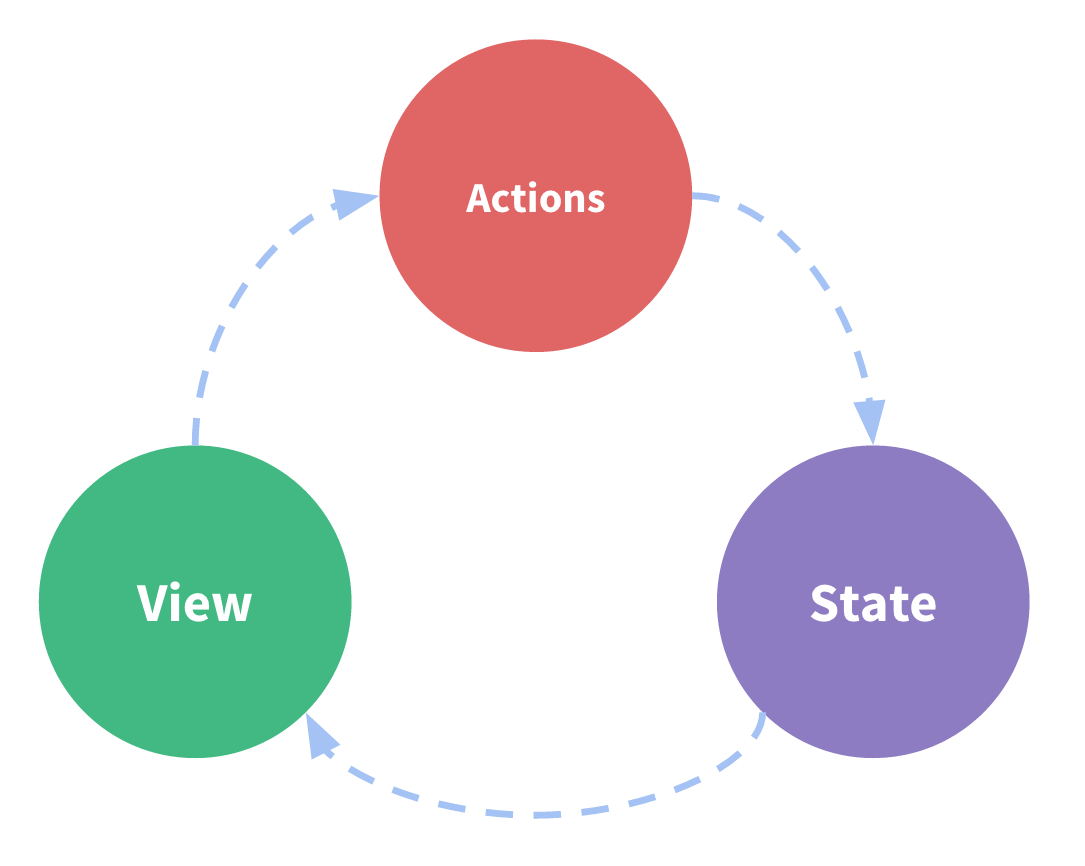
\includegraphics[scale=0.2]{pattern.png}
    \end{columns}
\end{frame}
\subsection{Use Case}
\begin{frame}
    \frametitle{Use Case}
    \begin{block}{Long Term vs. Short Term Productivity}
        \begin{center}
            Flux libraries (=Vuex) are like glasses: you’ll know when you need them.
            \\-Dan Abramov

        \end{center}
    \end{block}
\end{frame}

\section{Installation/Nutzung}
\subsection{Download}
\begin{frame}[fragile]
    \frametitle{Download}
    Manuelle Installation
    \begin{itemize}
        \item nicht empfohlen
    \end{itemize}
    Paketmanager
    \begin{itemize}
        \item npm
        \item yarn
    \end{itemize}
\end{frame}
\subsection{Registrierung}
\begin{frame}
    \frametitle{Registrierung}
    Vuex-Datei: $"$store.js$"$ \\~\\
    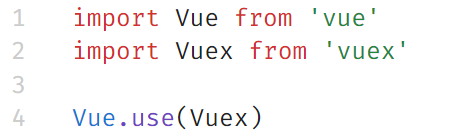
\includegraphics[scale=0.4]{registrierung.png}
\end{frame}
\subsection{Store einbinden}
\begin{frame}
    \frametitle{Store einbinden}
    $"$main.js$"$ \\~\\
    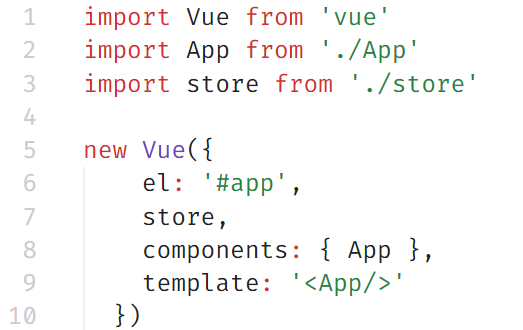
\includegraphics[scale=0.4]{einbinden.png}
\end{frame}
\subsection{Zugriff}
\begin{frame}
    \frametitle{Zugriff}
    \begin{itemize}
        \item \$store-Objekt
    \end{itemize}
\end{frame}
\section{Core Concepts}
\subsection{State}
\begin{frame}
    \frametitle{State}
\end{frame}
\subsection{Getters}
\begin{frame}
    \frametitle{Getters}
\end{frame}
\subsection{Mutations}
\begin{frame}
    \frametitle{Mutations}
\end{frame}
\subsection{Actions}
\begin{frame}
    \frametitle{Actions}
\end{frame}
\subsection{Modules}
\begin{frame}
    \frametitle{Modules}
\end{frame}
\begin{frame}
    \frametitle{Quellen}
\end{frame}
\end{document}